%%% Kapitel �ber Diagonalisierung von H, Ergebnisse und Diskussion
%%% Time-stamp: <1999-03-04 13:59:35 ralf>

\chapter{Ergebnisse und Diskussion}
\label{cha:ergebnisse}

%%%%%%%%%%%%%%%%%%%%%%%%%%%%%%%%%%%%%%%%%%%%%%%%
\section{Diagonalisieren des Hamilton-Operators}
\label{sec:diag}

Die Diagonalisierung des \kdotp-Hamilton-Operators \eqref{eq:k.p-H} wollen wir
in mehreren Schritten vornehmen. Die Idee dabei ist, da"s wir zun"achst
Gl.~\eqref{eq:k.p-H} f"ur $k=0$ diagonalisieren. Dadurch erhalten wir neue
Basisfunktionen, die sich als Linearkombination der alten Basisfunktionen
darstellen lassen, so da"s wir die \kdotp-Wechselwirkungen zwischen diesen
neuen Basisfunktionen angeben k"onnen. Danach k"onnen wir dann diese
Kopplungen in zweiter Ordnung St"orungstheorie behandeln, um die effektiven
Massen zu erhalten.


%%%%%%%%%%%%%%%%%%%%%%%
\subsection{Entkopplung von Valenz- und Leitungsband}
\label{sec:V15}

In Gl.~\eqref{eq:V15-V11} haben wir gesehen, da"s \V{15}, verglichen mit
den dazugeh"origen Energienennern, das Matrixelement mit dem geringsten Effekt
ist. Wie wir noch sehen werden, gilt $|\V{11}| \approx 200$~meV f"ur die
h"ochstgeordneten Proben, die im Experiment bisher gefunden wurden. Setzen wir
aber nun die Werte aus Tab.~\ref{tab:Em*P} ein, so erhalten wir, da"s auch
$|\V{15}| \approx 200$~meV ist und damit eine Gr"o"senordnung kleiner als
der dazugeh"orige Energienenner. Dies rechtfertigt es, diese Kopplung
st"orungstheoretisch zu behandeln.

Dabei wollen wir L"owdin-St"orungstheorie \cite{lowd:51} verwenden, wie wir
sie in Kap.~\ref{sec:standard-k.p} beschrieben haben.  Da wir hier eine
Entkopplung von Valenz- und Leitungsband durchf"uhren m"ochten, bedeutet dies,
da"s wir einmal die Leitungsb"ander als Gruppe \raum{A} betrachten und die
Valenzb"ander als Gruppe \raum{B} und dann diese Rollen vertauschen.

F"uhren wir dies f"ur den Hamilton-Operator \eqref{eq:k.p-H} durch, so m"ussen
wir nur folgende Energien ab"andern, um die Kopplung zwischen Valenz- und
Leitungsband in zweiter Ordnung zu beseitigen:
%
%\begin{subequations}
%\label{eq:E-shift}
\begin{eqnarray*}
%  \label{eq:EL-shift}
  \tilde{E}_{\text{Lc}} &=& E_{\text{Lc}} + \frac{|\V{15}|^{2}}{E_{\text{Lc}}}\\
%  \label{eq:EG-shift} 
  \tilde{E}_{\Gamma \text{v}}^{z} &=& - \frac{|\V{15}|^{2}}{E_{\text{Lc}}}
\end{eqnarray*}
%\end{subequations}
%
Die schwache Beimischung von \LCB-Anteilen zum \GVBz-Zustand und umgekehrt
soll im folgenden vernachl"assigt werden. 

Der gro"se Vorteil bei diesem Zugang ist, da"s wir nur den Betrag von \V{15}
ben"otigen, nicht aber dessen Vorzeichen. Damit haben wir die Anzahl der
M"oglichkeiten, die wir diskutieren m"ussen, auf zwei reduziert. Entweder haben
\V{11} und \V{35} gleiches Vorzeichen, oder verschiedenes. Der Nachteil ist,
da"s die Aussagekraft unseres Modells f"ur sehr hohen Ordnungsgrad nachl"a"st. 



%%%%%%%%%%%%%%%%%%%%%%
\subsection{Zwei-Niveau-Systeme}
\label{sec:2niveau}

Der n"achste Schritt ist die Diagonalisierung bez"uglich \V{11} und \V{35},
die einfach ist, da es sich dabei im Leitungs- und Valenzband um zwei
Zwei-Niveau-Systeme  handelt.

Im Leitungsband erhalten wir dadurch die Zust"ande
%
\begin{subequations}
\label{eq:CB-V}
\begin{eqnarray}
  \label{eq:GCB-V}
  \ket{\bGCB (\GCB)} &=& \alpha_{\text{c}} \ket{\GCB} + \beta_{\text{c}}
  \ket{\LCB}  \\
  \label{eq:LCB-V}
  \ket{\bGCB (\LCB)} &=& \beta_{\text{c}} \ket{\GCB} - \alpha_{\text{c}}
  \ket{\LCB}
\end{eqnarray}
\end{subequations}
%
mit den Eigenenergien
%
\begin{equation}
  \label{eq:E-CB-V}
  E_{\text{c}}^{(1/2)} = \frac{E_{\Gamma \text{c}} + \tilde E_{\text{Lc}}}{2}
  \mp \sqrt{\left( \frac{E_{\Gamma \text{c}} - \tilde E_{\text{Lc}}}{2}
  \right)^{2} + |\V{11}|^{2} } .
\end{equation}
%
Au"serdem gilt
%
\begin{subequations}
\label{eq:koeffCB}
\begin{eqnarray}
  \label{eq:alphaCB}
  \alpha_{\text{c}} &=& \frac{\V{11}}{\sqrt{\left( E_{\Gamma \text{c}} -
        E_{\text{c}}^{(1)} \right)^{2} + |\V{11}|^{2} }} \\
  \label{eq:betaCB}
  \beta_{\text{c}} &=& \frac{E_{\text{c}}^{(1)} - E_{\Gamma \text{c}}}
  {\sqrt{\left( E_{\Gamma \text{c}} - E_{\text{c}}^{(1)} \right)^{2} +
      |\V{11}|^{2} }} .
\end{eqnarray}
\end{subequations}
%
Dabei ist $E_{\text{c}}^{(1)}$ die Eigenenergie zu \ket{\bGCB (\GCB)} und
bezieht sich auf das Minuszeichen in Gl.~\eqref{eq:E-CB-V}.

Im Valenzband erhalten wir\footnote{Hier f"ur \bGVBx, analoges gilt auch f"ur
  \bGVBy} 
%
\begin{subequations}
\label{eq:VB-V}
\begin{eqnarray}
  \label{eq:GVB-V}
  \ket{\bGVBx (\GVBx)} &=& \alpha_{\text{v}} \ket{\GVBx} + \beta_{\text{v}}
  \ket{\LVBx}  \\
  \label{eq:LVB-V}
  \ket{\bGVBx (\LVBx)} &=& \beta_{\text{v}} \ket{\GVBx} - \alpha_{\text{v}}
  \ket{\LVBx}
\end{eqnarray}
\end{subequations}
%
mit den Eigenenergien
%
\begin{equation}
  \label{eq:E-VB-V}
  E_{\text{v}}^{(1/2)} = \frac{E_{\text{Lv}}}{2} \pm 
  \sqrt{\left( \frac{E_{\text{Lv}}}{2} \right)^{2} + |\V{35}|^{2} } .
\end{equation}
%
Au"serdem gilt
%
\begin{subequations}
\label{eq:koeffVB}
\begin{eqnarray}
  \label{eq:alphaVB}
  \alpha_{\text{v}} &=& \frac{\V{35}}
  {\sqrt{ {E_{\text{v}}^{(1)}}^{2} + |\V{35}|^{2} }} \\
  \label{eq:betaVB}
  \beta_{\text{v}} &=& \frac{E_{\text{v}}^{(1)}}
  {\sqrt{ {E_{\text{v}}^{(1)}}^{2} + |\V{35}|^{2} }} .
\end{eqnarray}
\end{subequations}
%
Dabei ist $E_{\text{v}}^{(1)}$ die Eigenenergie zu \ket{\bGVBx (\GVBx)} und
bezieht sich auf das Pluszeichen in Gl.~\eqref{eq:E-VB-V}.


%%%%%%%%%%%%%%%%%%%%%%%%
\subsection{Der neue \kdotp-Hamilton-Operator}
\label{sec:neu-k.p-H}


%%%%%%%%%%%% Neuer gesamt k.p Hamilton-Operator
%\begin{floateqnum}
\begin{sidewaysfloateqnum}
\begin{equation}
\label{eq:neu-k.p-H}
\caption{\kdotp-Hamilton-Operator bez"uglich Basis, die Ordnungspotential diagonalisiert.}
\renewcommand{\arraystretch}{1.6}
\op{H_{\bar \Gamma}} = \left(
\begin{array}{c|cc|c||c|cc}
  \raisebox{2.0em}[0ex][0ex]{\ket{\bGCB  (\GCB)}} 
& \raisebox{2.0em}[0ex][0ex]{\ket{\bGVBx (\GVBx)}} 
& \raisebox{2.0em}[0ex][0ex]{\ket{\bGVBy (\GVBy)}} 
& \raisebox{2.0em}[0ex][0ex]{\ket{\bGVB{1} (\GVBz)}} 
& \raisebox{2.0em}[0ex][0ex]{\ket{\bGCB  (\LCB)}} 
& \raisebox{2.0em}[0ex][0ex]{\ket{\bGVBx (\LVBx)}} 
& \raisebox{2.0em}[0ex][0ex]{\ket{\bGVBy (\LVBy)}} \\[-4ex]
%%%%%%%%%%%
\begin{array}[c]{c} E_{\text{c}}^{(1)} + \frac{\hbar^{2}}{2m} k^{2}\\
  + {\beta_{\text{c}}}^{2} G k_{z}^{2}
  \end{array} 
& i P_{1} k_{x} 
& i P_{1} k_{y} 
& i \pri{P_{1}} k_{z} 
& 0 
& - i P_{2} k_{x} 
& - i P_{2} k_{y} \\
\hline
%%%%%%%%%%%
  -i P_{1} k_{x} 
& E_{\text{v}}^{(1)} + \frac{\hbar^{2}}{2m}k ^{2} 
& 0 
& 0 
& - i P_{2} k_{x} 
& 0 
& 0 \\
%%%%%%%%%%%
  -i P_{1} k_{y} 
& 0 
& E_{\text{v}}^{(1)} + \frac{\hbar^{2}}{2m} k^{2} 
& 0 
& - i P_{2} k_{y}
& 0 
& 0   \\
%%%%%%%%%%%
\hline
  -i \pri{P_{1}} k_{z} 
& 0 
& 0 
& \tilde E^{z}_{\Gamma \text{v}} + \frac{\hbar^{2}}{2m} k^{2} 
& - i \pri{P_{2}} k_{z}
& 0 
& 0 \\
\hline\hline
%%%%%%%%%%%
0 
& i P_{2} k_{x}
& i P_{2} k_{y}
& i \pri{P_{2}} k_{z}
& \begin{array}[c]{c} E_{\text{c}}^{(2)} + \frac{\hbar^{2}}{2m} k^{2}\\
  + {\alpha_{\text{c}}}^{2} G k_{z}^{2}
  \end{array} 
& i P_{1} k_{x} 
& i P_{1} k_{y}\\
%%%%%%%%%%%
\hline
i P_{2} k_{x} 
& 0 
& 0 
& 0 
& -i P_{1} k_{x} 
& E_{\text{v}}^{(2)} + \frac{\hbar^{2}}{2m} k^{2} 
& 0 \\
%%%%%%%%%%%
i P_{2} k_{y}
& 0 
& 0 
& 0 
& -i P_{1} k_{y} 
& 0 
& E_{\text{v}}^{(2)} + \frac{\hbar^{2}}{2m} k^{2} \\
\end{array} \right)
\renewcommand{\arraystretch}{0.625}
\end{equation}
%\end{floateqnum}
\end{sidewaysfloateqnum}
%%%%%%%%%%%%%%%%%%%%%%%%%%%%%%%

Verwenden wir nun die neuen Basisfunktionen Gln.~\eqref{eq:CB-V} und
\eqref{eq:VB-V}, die diagonal bez"uglich der Potentialmatrixelemente sind, und
betrachten die \kdotp-Matrix \eqref{eq:k.p-H} in dieser Basis, so erhalten wir
eine neue Matrix, die in Gl.~\eqref{eq:neu-k.p-H} (siehe
S.~\pageref{eq:neu-k.p-H}) angegeben ist. Dabei wurden folgende Abk"urzungen
verwendet:
%
\begin{subequations}
\label{eg:P1-P2'}
\begin{eqnarray}
  \label{eq:P1}
  P_{1} &=& (\alpha_{\text{v}} \alpha_{\text{c}} + \beta_{\text{v}}
  \beta_{\text{c}}) \PG \\
  \label{eq:P2}
  P_{2} &=& (\alpha_{\text{v}} \beta_{\text{c}} - \beta_{\text{v}}
  \alpha_{\text{c}}) \PG \\
  \label{eq:P1'}
  \pri{P_{1}} &=& \alpha_{\text{c}} \PG \\
  \label{eq:P2'}
  \pri{P_{2}} &=& \beta_{\text{c}} \PG
\end{eqnarray}
\end{subequations}
%
Daraus erhalten wir nun direkt die effektiven Massen in den untersten beiden
Leitungsb"andern, indem wir Gl.~\eqref{eq:neu-k.p-H} in zweiter Ordnung
St"orungstheorie bez"uglich $k$ diagonalisieren. 

F"ur den \bGCB (\GCB)-Zustand erhalten wir:
%
\begin{subequations}
\label{eq:m*-GCB-G}
\begin{eqnarray}
  \label{eq:m*-GCB-G.parallel}
  \frac{m}{m_{\parallel}^{(1)}} &=& 1 + \frac{2m}{\hbar^{2}} \left(
    \beta_{\text{c}}^{2} G + \frac{|\pri{P_{1}}|^{2}}{E_{\text{c}}^{(1)} -
      \tilde E^{z}_{\Gamma \text{v}}} \right) \\
  \label{eq:m*-GCB-G.senkrecht}
  \frac{m}{m_{\perp}^{(1)}} &=& 1 + \frac{2m}{\hbar^{2}} \left(
    \frac{|P_{1}|^{2}}{E_{\text{c}}^{(1)} - E^{(1)}_{\text{v}}} +
    \frac{|P_{2}|^{2}}{E_{\text{c}}^{(1)} - E^{(2)}_{\text{v}}} \right)
\end{eqnarray}
\end{subequations}
%
Dabei gilt $m_{\parallel}^{(1)}$ f"ur die Richtung parallel zur
Ordnungsrichtung, d.~h.\ der $[111]$-Richtung , $m_{\perp}^{(1)}$ senkrecht zu
dieser.  

F"ur das \bGCB (\LCB)-Niveau ergibt sich
%
\begin{subequations}
\label{eq:m*-GCB-L}
\begin{eqnarray}
  \label{eq:m*-GCB-L.parallel}
  \frac{m}{m_{\parallel}^{(2)}} &=& 1 + \frac{2m}{\hbar^{2}} \left(
    \alpha_{\text{c}}^{2} G + \frac{|\pri{P_{2}}|^{2}}{E_{\text{c}}^{(2)} -
      \tilde E^{z}_{\Gamma \text{v}}} \right) \\
  \label{eq:m*-GCB-L.senkrecht}
  \frac{m}{m_{\perp}^{(2)}} &=& 1 + \frac{2m}{\hbar^{2}} \left(
    \frac{|P_{1}|^{2}}{E_{\text{c}}^{(2)} - E^{(2)}_{\text{v}}} +
    \frac{|P_{2}|^{2}}{E_{\text{c}}^{(2)} - E^{(1)}_{\text{v}}} \right)
\end{eqnarray}
\end{subequations}
%
mit entsprechenden Bedeutungen von $m_{\parallel}^{(2)}$ und $m_{\perp}^{(2)}$.

An dieser Stelle sehen wir auch, wie die in Kap.~\ref{sec:phase} diskutierten
Phasen der Matrixelemente eingehen. Denn zum einen h"angen $\alpha_{\text{c}}$
und $\alpha_{\text{v}}$ direkt vom Vorzeichen der Potentialmatrixelemente
\V{11} bzw.\ \V{35} ab. Zum anderen geht auch ein, da"s $\PG = \PL$ gilt. Es
f"allt allerdings auf, da"s die beiden Massen parallel zur Ordnungsrichtung
$m^{(1/2)}_{\parallel}$ nicht von den Phasenbeziehungen abh"angen, da hier von
phasenabh"angigen Gr"o"sen nur Betragsquadrate eingehen.


%%%%%%%%%%%%%%%%%%%%%%%%%%%%%%%%%%%%%%%
\section{Ergebnisse}
\label{sec:ergeb}

Die im vorhergehenden Abschnitt abgeleiteten Formeln lassen sich f"ur
verschiedene Werte von \V{11} numerisch l"osen. Da \V{11} der einzige freie
Parameter in unserem Modell ist, werden wir die Ergebnisse solch einer
Rechnung auch in Abh"angigkeit von \V{11} darstellen. Experimentell ist es
aber kaum m"oglich, 
\V{11} zu bestimmen, weshalb wir in Anhang~\ref{cha:ergeb-BGR} diese Ergebnisse
auch als Funktion der Bandl"uckenreduzierung zeigen.

%%%%%%%%%%%%%%
\subsection{Energieeigenwerte}
\label{sec:energie}

Zun"achst wollen wir die Bandkantenenergien betrachten, wie sie sich aus
unserer Rechnung ergeben. Abb.~\ref{fig:energie}(a) zeigt, wie sich
Bandl"uckenreduzierung $\Delta E_{\text{BGR}}$, Kristallfeldaufspaltung
$\Delta_{\text{CF}}$ und "Anderung $\Delta E_{\Gamma \rightarrow \text{L}}$ der
"Ubergangsenergie $\bGVB{3}(\GVB) \rightarrow \bGCB (\LCB)$ als Funktion von
\V{11} verhalten. Dabei wird \V{11} als positiv angenommen, da die hier
diskutierten Ph"anomene nicht von den absoluten Phasen der Matrixelemente
abh"angen. Das liegt unter anderen daran, da"s ein Austausch von Ga- und
In-reichen Lagen an der Physik der geordneten Struktur nichts "andern kann,
aber zu einem Vorzeichenwechsel bei den Matrixelementen f"uhrt.

\begin{figure}[htb]
  \centering 
  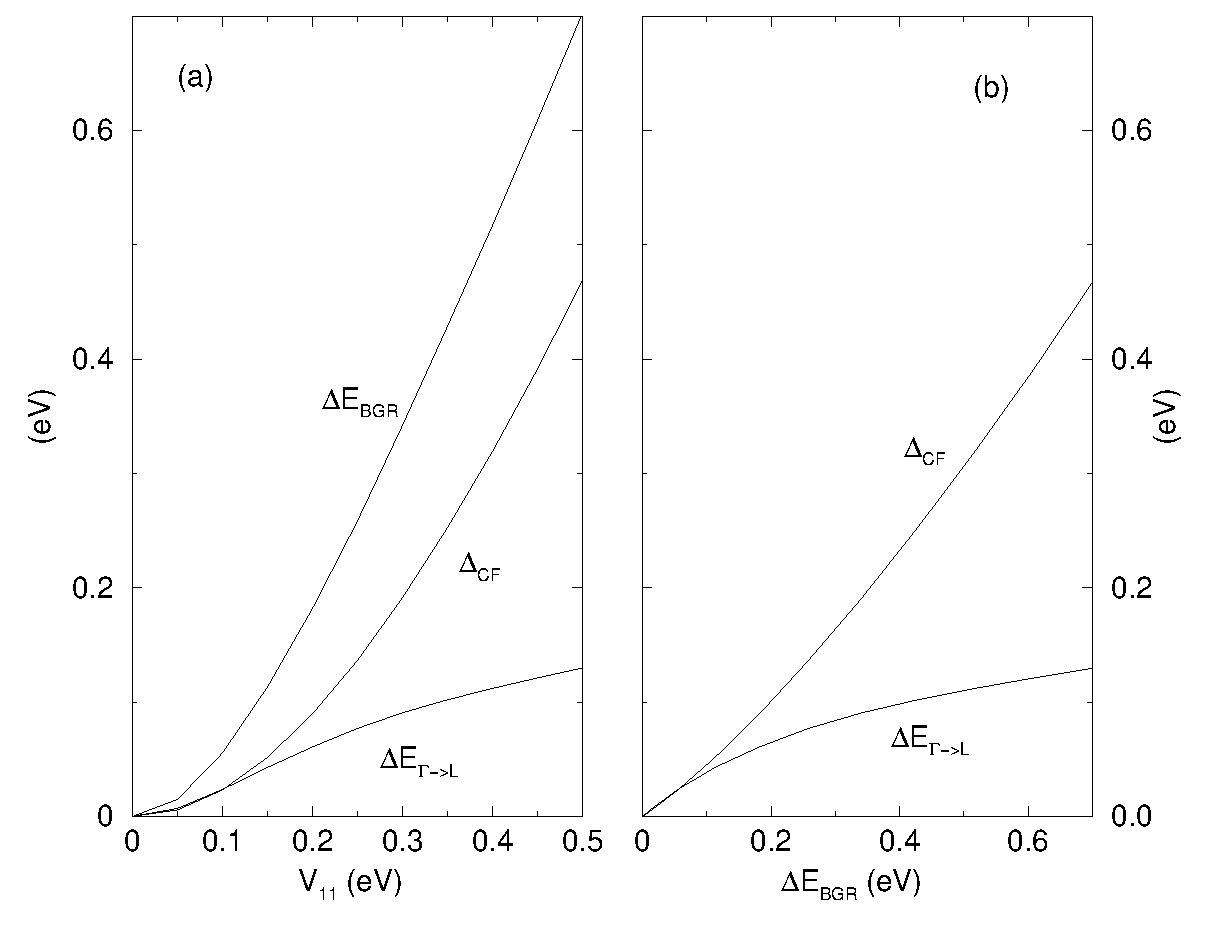
\includegraphics[width=\textwidth]{BGR.CF.eps}
  \caption{(a) Bandl"uckenreduzierung $\Delta E_{\text{BGR}}$,
  Kristallfeldaufspaltung $\Delta_{\text{CF}}$ und "Anderung $\Delta E_{\Gamma
  \rightarrow \text{L}}$ der "Ubergangsenergie $\bGVB{3}(\GVB) \rightarrow
  \bGCB (\LCB)$ als Funktion von \V{11}. (b) Kristallfeldaufspaltung
  $\Delta_{\text{CF}}$ und "Anderung $\Delta E_{\Gamma \rightarrow \text{L}}$
  der "Ubergangsenergie $\bGVB{3}(\GVB) \rightarrow \bGCB (\LCB)$ als Funktion
  der Bandl"uckenreduzierung $\Delta E_{\text{BGR}}$.}
  \label{fig:energie}
\end{figure}

Die Betrachtung der Bandkantenergien ist notwendig, weil wir sonst nicht
wissen k"onnen, wie gro"s unsere Matrixelemente sein m"ussen, um einen
Kristall mit einem bestimmten Ordnungsgrad zu beschreiben.

An den h"ochstgeordneten Proben, die heute hergestellt werden k"onnen, werden
typischerweise Bandl"uckenreduzierungen von $100 \dots 150$~meV gemessen
\cite{ezdm:97,kipp:97}. Solche Werte erhalten wir f"ur $\V{11} = 150 \dots
200$~meV. $\V{11} = 0 \dots 200$~meV ist also der Bereich, der realistische
Proben beschreibt. Wie bereits in Kap.~\ref{sec:V15} erw"ahnt,
ist dies auch der Bereich, in dem die St"orungstheorie f"ur \V{15}
gerechtfertigt ist. Vorhersagen f"ur im Experiment beobachtete Proben
sind also m"oglich. Bei Aussagen "uber st"arker geordnete Proben ist
zudem zu beachten, da"s Gln.~\eqref{eq:zeta} und \eqref{eq:theta} nicht
mehr erf"ullt sein m"ussen, was die Verh"altnisse zwischen den
Potentialmatrixelementen ver"andern w"urde.

Wei und Zunger \cite{wezu:98} geben 430~meV als theoretische
Bandl"uckenabsenkung der ideal geordneten Struktur an. Wie aus
Abb.~\ref{fig:energie} ersichtlich, erhalten wir diesen Wert f"ur $\V{11}
\approx 350$~meV. Wir werden uns deshalb bei weiteren Darstellungen auf den
Bereich zwischen 0~meV und 350~meV f"ur \V{11} beschr"anken. Diese
Abbildungen, die Impulsmatrixelemente und effektive Massen als Funktion von
\V{11} zeigen, werden so aufgebaut sein, da"s auf der linken Seite der Fall
gleichen Vorzeichens von \V{11} und \V{35} zu sehen ist ("`Phase: +1"'), auf
der rechten Seite der Fall verschiedenen Vorzeichens ("`Phase: -1"').

Wie bereits in Kap.~\ref{sec:betrag} erw"ahnt, gilt $\V{11} \propto \eta$,
wenn das Ordnungspotential mit Hilfe der VCA modelliert wird. Laks, Wei und
Zunger \cite{lwz:92} trafen die allgemeine Vorhersage, da"s physikalische
Eigenschaften langreichweitig geordneter Systeme in Abh"angigkeit von
Ordnungsgrad $\eta$ im wesentlichen wie $\eta^{2}$ skalieren. Wenn also
$\V{11} \propto \eta$ gilt, so l"a"st dies eine $\V{11}^{\; 2}$-Abh"angigkeit
erwarten. F"ur $\Delta E_{\text{BGR}}$ und $\Delta_{\text{CF}}$ ist dies auch
gut erf"ullt, wie Abb.~\ref{fig:energie}(a) und der nahezu lineare
Zusammenhang zwischen diesen Gr"o"sen in Abb.~\ref{fig:energie}(b) zeigt. Doch
f"ur $\Delta E_{\Gamma \rightarrow \text{L}}$ ist dies nur f"ur kleine \V{11}
erf"ullt. Da"s dies f"ur kleine \V{11} gilt, ist leicht "uber die 2. Ordnung
einer St"orungstheorie f"ur kleines \V{11} zu verstehen. Die f"ur gr"o"sere
Matrixelemente auftretenden Fehler scheinen sich f"ur $\Delta E_{\text{BGR}}$
und $\Delta_{\text{CF}}$ nahezu zu kompensieren, w"ahrend sie sich f"ur
$\Delta E_{\Gamma \rightarrow \text{L}}$ verst"arken.
 

%%%%%%%%%%%%%%
\subsection{Impulsmatrixelemente}
\label{sec:impulsme}

In Abb.~\ref{fig:P-me} sind die Impulsmatrixelemente, die in
Gl.~\eqref{eq:neu-k.p-H} auftreten, als Funktion von \V{11} zu sehen. Es f"allt
auf, da"s die Kurven f"ur $|\pri{P_{1}}|^{2}$ und $|\pri{P_{2}}|^{2}$
unabh"angig vom relativen Vorzeichen von \V{11} und \V{35} sind. Dies
l"a"st sich leicht verstehen, da in Gln.~\eqref{eq:P1'} und \eqref{eq:P2'}
keine Summen von Entwicklungskoeffizienten aus den Zwei-Niveau-Systemen
auftreten. Denn diese Summen, wie sie in Gln.~\eqref{eq:P1} und \eqref{eq:P2}
auftreten, f"uhren zu konstruktiver oder destruktiver "Uberlagerung der
\kdotp-Wechselwirkung zwischen $\Gamma$-Punkts-Wellenfunktionen einerseits und
L-Punkts-Wellenfunktionen andererseits. Haben z.~B.\ \V{11} und \V{35} das
gleiche Vorzeichen, so gilt dies auch f"ur $\alpha_{\text{c}}$ und
$\alpha_{\text{v}}$ [Gln.~\eqref{eq:alphaCB} und \eqref{eq:alphaVB}]. Dagegen
haben $\beta_{\text{c}}$ und $\beta_{\text{v}}$ immer verschiedenes Vorzeichen
[Gln. \eqref{eq:betaCB} und \eqref{eq:betaVB}]. Damit ergibt sich aus
Gl.~\eqref{eq:P1} ein stark abnehmendes $P_{1}$, wie es auch in
Abb.~\ref{fig:P-me} f"ur den Fall positiver relativer Phase zu sehen
ist.%\marginpar{St"orungstheorie...?}

\begin{figure}[htb]
  \centering 
  \includegraphics[width=\textwidth]{P2.eps}
  \caption{Betragsquadrat der Impulsmatrixelemente aus Gl.~\eqref{eq:neu-k.p-H}
  f"ur positives und negatives relatives Vorzeichen von \V{11} und \V{35} in
  Einheiten von $|\PG|^{2}$.} 
  \label{fig:P-me}
\end{figure}

Dabei spielen die Impulsmatrixelemente nicht nur f"ur die Bandkr"ummungen eine
entscheidende Rolle. Sie sind auch f"ur die St"arke optischer Dipol"uberg"ange
verantwortlich \cite{kitt:67}. So ist die Wahrscheinlichkeit eines "Ubergangs
$\bGVB{3} (\GVB) \rightarrow \bGCB (\GCB)$ proportional zu $|P_{1}|^{2}$, wenn
das Licht senkrecht zur Ordnungsrichtung polarisiert ist. F"ur die gleiche
Polarisationsrichtung beschreibt $|P_{2}|^{2}$ die Intensit"at des "Ubergangs
$\bGVB{3} (\GVB) \rightarrow \bGCB (\LCB)$. Dies erm"oglicht es, die relative
Phase von \V{11} und \V{35} zu bestimmen. Denn f"ur hochgeordnete Proben --
$\V{11} \approx 200$~meV -- sagt unsere Rechnung in etwa gleiche Intensit"at
f"ur diese "Uberg"ange voraus, wenn das relative Vorzeichen positiv ist. Ist
es negativ, so ist der "Ubergang $\bGVB{3} (\GVB) \rightarrow \bGCB (\LCB)$ um
etwa eine Gr"o"senordnung unterdr"uckt, wie aus Abb.~\ref{fig:P-me}
ersichtlich ist. Der letztere Fall beschreibt die im Experiment gefundenen
St"arken der Dipol"uberg"ange deutlich besser \cite{kksk:99}, so da"s wir mit
hoher Wahrscheinlichkeit davon ausgehen k"onnen, da"s das relative Vorzeichen
von \V{11} und \V{35} negativ ist. Da diese Bestimmung aber nicht vollst"andig
eindeutig ist, wollen wir trotzdem auch die Ergebnisse f"ur eine positive
relative Phase zeigen.

Wichtig sind diese Ergebnisse f"ur die Berechnung der
polarisations"-ab"-h"angigen Absorption \CuPt-geordneter \GaInP-Proben. In
bisherigen Rechnungen \cite{wezu:94-2,wezu:94} wurde immer von \emph{einem}
Dipolmatrixelement zwischen Zu"-st"an"-den im obersten Valenzband und im
untersten Leitungsband  ausgegangen. Dies gilt exakt aber nur im Grenzfall
verschwindender Ordnung, d.~h.\ kubischer Symmetrie. Denn vom Standpunkt der
Gruppentheorie aus betrachtet, gibt es keinen Grund warum
%
\begin{displaymath}
  \Matrixel{\bGCB (\GCB)}{\op{p_{z}}}{\bGVB{1} (\GVBz)} \stackrel{?}{=} 
  \Matrixel{\bGCB (\GCB)}{\op{p_{x}}}{\bGVB{3} (\GVBx)}
\end{displaymath}
%
gelten sollte, da \bGVB{1} (\GVBz) und \bGVB{3} (\GVBx) zu verschiedenen
Darstellungen der \Cdv\ geh"oren, und auch \op{p_{z}} und \op{p_{x}} sich
verschieden transformieren. Die in Abb.~\ref{fig:P-me} zu sehenden Ergebnisse
zeigen nun, da"s diese Ungleichheit nicht nur gilt, sondern da"s sie bereits
f"ur realistischen Ordnungsgrad nicht zu vernachl"assigen ist. Bei der
Auswertung polarisationsabh"angiger Messungen an "Uberg"angen vom
Va"-lenz"-band-Maximum zum \bGCB (\LCB) Zustand ist die Ber"ucksichtigung
dieser Ungleichheit besonders wichtig. Denn das Va"-lenz"-band-Maximum
enth"alt auf Grund der Spin-Bahn-Wechselwirkung sowohl \bGVB{3} als auch
\bGVB{1} Zust"ande, und die relativen Unterschiede zwischen $|P_{2}|^{2}$ und
$|\pri{P_{2}}|^{2}$ sind weit gr"o"ser als zwischen $|P_{1}|^{2}$ und
$|\pri{P_{1}}|^{2}$.

Das in Abb.~\ref{fig:P-me} f"ur eine positive Phase zu sehende Verhalten von
$|P_{1}|^{2}$ und $|\pri{P_{2}}|^{2}$ bzw.\ $|P_{2}|^{2}$ und
$|\pri{P_{1}}|^{2}$ k"onnte nahelegen, da"s sie sich einem gemeinsammen
Grenzwert ann"ahern. Tats"achlich schneiden sie sich nur und laufen danach
wieder auseinander. Da"s dieser Schnittpunkt so nahe an der oberen Grenze des
f"ur uns interessanten Bereichs liegt, erscheint zuf"allig zu sein.



%%%%%%%%%%%%%%
\subsection{Effektive Massen von \bGCB (\GCB)}
\label{sec:m*-GCB}

In Abb.~\ref{fig:m*-GCB} sind nun die Vorhersagen unseres Modells f"ur die
Ordnungsabh"angigkeit der effektiven Masse des \bGCB (\GCB)-Niveaus, d.~h.\
des untersten Leitungsbandes, zu sehen, wie sie sich aus
Gln.~\eqref{eq:m*-GCB-G} ergeben. 

\begin{figure}[htb]
  \centering
  \includegraphics[width=\textwidth]{masses.G.eps}
  \caption{Effektive Massen von \bGCB (\GCB) f"ur positives und negatives
    relatives Vorzeichen von \V{11} und \V{35}.} 
  \label{fig:m*-GCB}
\end{figure}

"Ahnlich wie in Abb.~\ref{fig:P-me} f"allt auf, da"s eine der Gr"o"sen -- hier
die effektive Masse parallel zur Ordnungsrichtung $m_{\parallel}$ --
unabh"angig vom relativen Vorzeichen der Potentialmatrixelemente ist. Dies
k"onnen wir wiederum darauf zur"uckf"uhren, da"s in
Gl.~\eqref{eq:m*-GCB-G.parallel} keine Summen von Entwicklungskoeffizienten
aus den Zwei-Niveau-Systemen auftreten. F"ur den Anstieg in $m_{\parallel}$
ist die Mischung von \GCB- mit \LCB-Zust"anden verantwortlich, da sie
$|\pri{P_{1}}|$ gegen"uber \PG\ verkleinert und die sehr flache Dispersion des
\LCB-Niveaus in $[111]$-Richtung beigemischt wird.

Dagegen verh"alt sich $m_{\perp}$ sehr unterschiedlich, wenn sich die relative
Phase von \V{11} zu \V{35} "andert. Dies k"onnen wir leicht durch das
unterschiedliche Verhalten von $|P_{1}|^{2}$ und $|P_{2}|^{2}$
verstehen. Unabh"angig von der relativen Phase verkleinern sich die
Energienenner in Gl.~\eqref{eq:m*-GCB-G.senkrecht}. Doch im Falle positiver
Phase beobachten wir einen starken Abfall in $|P_{1}|^{2}$ (siehe
Abb.~\ref{fig:P-me}), der sich nicht durch den Anstieg in $|P_{2}|^{2}$
kompensieren l"a"st, da das \bGVB{3} (\LVB)-Niveau etwa 1~eV tiefer als das
\bGVB{3} (\GVB)-Niveau liegt. F"ur negative Phase "andern sich die
Impulsmatrixelemente viel weniger, so da"s die Bandl"uckenreduzierung hier
voll zutragen kommt und eine stark ausgepr"agt Anisotropie der effektiven
Masse von $(m_{\parallel} - m_{\perp})/m_{\Gamma}^{\text{c}} = 0,489$ f"ur
$\V{11} = 350$~meV bzw. 0,217 f"ur $\V{11} = 150$~meV zu beobachten ist.

Wie wir im letzten Abschnitt erkl"art haben, beschreibt eine negative relative
Phase die beobachtete Absorption deutlich besser, als eine positive Phase, so
da"s die effektiven Massen f"ur negative Phase als unsere Vorhersage f"ur
teilgeordnetes \GaInP\ anzusehen sind. Vergleichen wir diese Ergebnisse mit
Dichtefunktionaltheorie Rechnungen von Franceschetti \emph{et al.}
\cite{fwz:95}, so stellen wir eine qualitative und teilweise auch quantitative
"Ubereinstimmung fest. So finden sie eine Anisotropie von 0,46 f"ur
vollst"andig geordnetes \GaInP, sehr nahe an unserem Wert von 0,489. Das
qualitative Bild einer Erh"ohung der effektiven Masse in Ordnungsrichtung und
einer Erniedrigung senkrecht dazu ist ebenfalls identisch. Nur die
Verh"altnisse verschieben sich etwas. Sie stellen nur eine sehr geringe
Reduktion der effektiven Masse senkrecht zur Ordnungsrichtung fest, w"ahrend
der Anstieg parallel zur Ordnungsrichtung ausgepr"agter ausf"allt. Dieser
Unterschied k"onnte auf die Methode, die bei der Korrektur des LDA-Fehlers
angewendet wurde, zur"uckzuf"uhren sein.

Das bisher einzige Experiment, das die Anisotropie der effektiven
Masse im untersten Leitungsband untersucht, wurde von Ernst \emph{et al.}
\cite{ezdm:97} durchgef"uhrt. Sie bestimmten die effektive Exzitonen-Masse
f"ur verschieden stark geordnete Proben mit Hilfe von
Photolumineszenz-Messungen im Magnetfeld. Auch sie fanden einen Anstieg
parallel zur 
Ordnungsrichtung und ein Absinken der effektiven Exzitonen-Masse senkrecht zu
ihr, stimmen also qualitativ mit den theoretische Vorhersagen "uberein. Ein
quantitativer Vergleich ist allerdings schwierig, da "uber die  "Anderungen in
den effektiven Massen der Valenzb"ander wenig bekannt ist.
 

%%%%%%%%%%%%%%
\subsection{Effektive Massen von \bGCB (\LCB)}
\label{sec:m*-LCB}

Die effektiven Massen, die sich aus Gln.~\eqref{eq:m*-GCB-L} ergeben, sind in
Abb.~\ref{fig:m*-LCB} dargestellt.  Auch hier ist die effektiven Masse
parallel zur Ordnungsrichtung $m_{\parallel}$ unabh"angig von der relativen
Phase der Potentialmatrixelemente. Die Erkl"arung f"ur dieses Verhalten ist
analog zu der im letzten Abschnitt pr"asentierten, nur die Rollen von $P_{1}$
und $P_{2}$ m"ussen vertauscht werden.  Der auff"alligsten Effekt, den wir
beobachten k"onnen, ist der starke Abfall in $m_{\parallel}$ von $1,7 m$ auf
unter $0,4 m$. Dies ist auf die Beimischung des \GCB-Zustandes
zur"uckzuf"uhren. Denn auf Grund dieser Beimischung besteht nun eine
\mbox{\kdotp}-Kopplung f"ur \vec{k} parallel zur Ordnungsrichtung zwischen dem
\bGCB (\LCB)-Zu"-stand und dem Valenzbandmaximum. Zuvor wurde $m_{\parallel}$
nur durch den Fernbandbeitrag $G$ bestimmt.

\afterpage{\clearpage
\begin{figure}[H]%[htb]
  \centering
  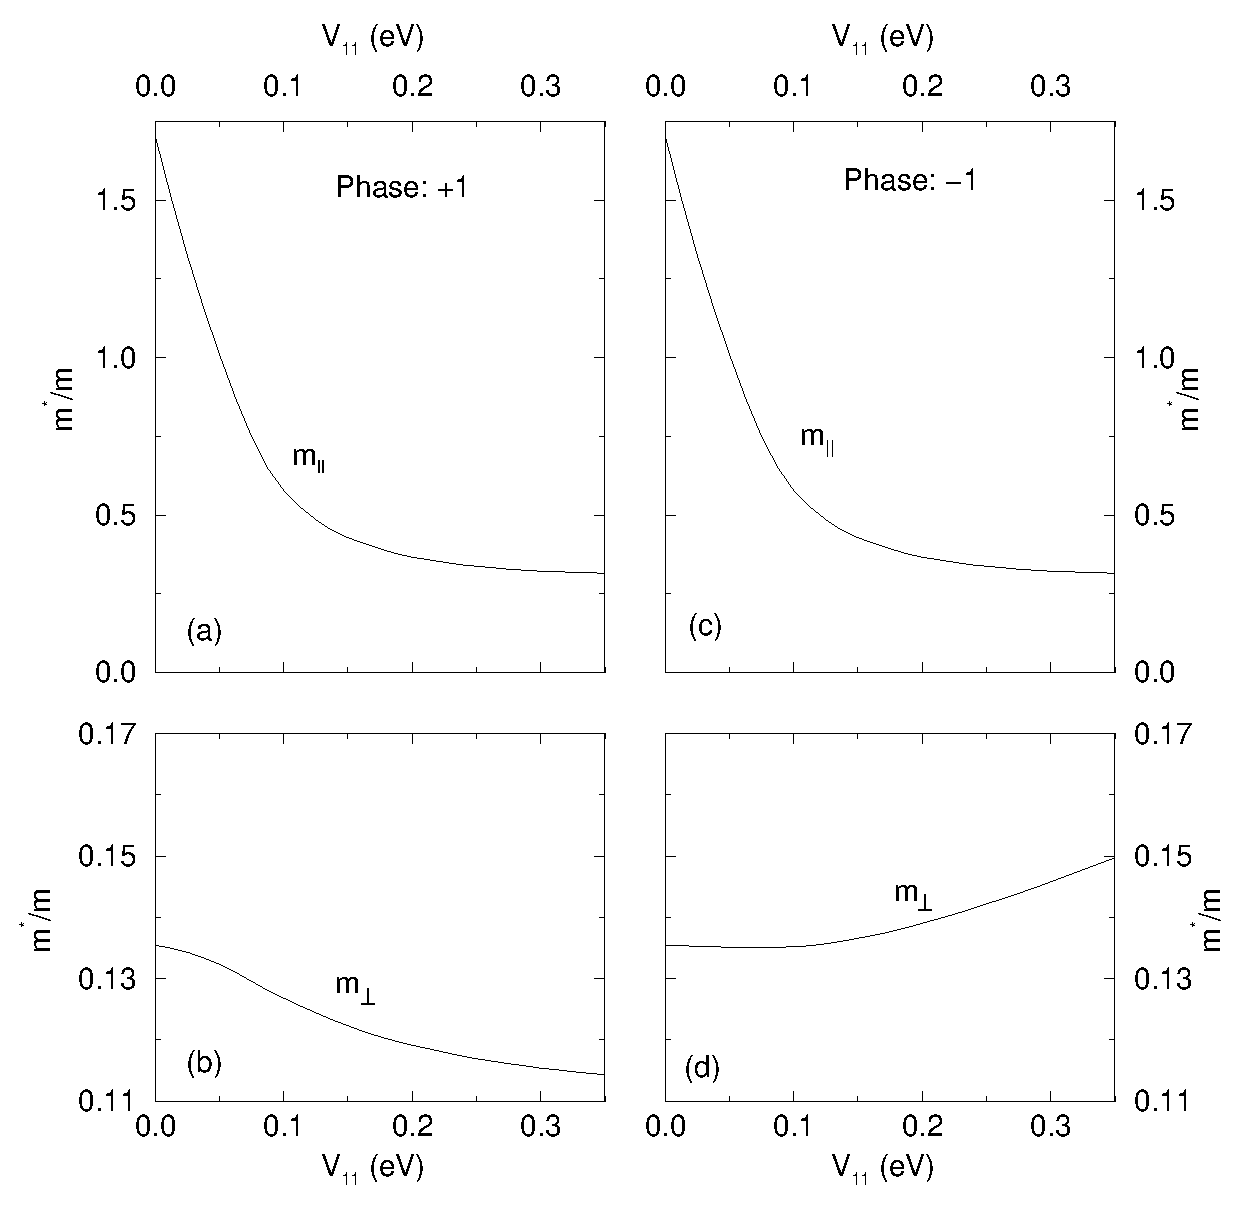
\includegraphics[width=\textwidth]{masses.L2.eps}
  \caption{Effektive Massen von \bGCB (\LCB) f"ur (a) und (b) positives sowie
  (c) und (d) negatives relatives Vorzeichen von \V{11} und \V{35}.} 
  \label{fig:m*-LCB}
\end{figure}
}


Die "Anderungen der effektiven Masse senkrecht zur Ordnungsrichtung
$m_{\perp}$ sind dagegen von "ahnlicher Gr"o"se wie die f"ur den \bGCB
(\GCB)-Zustand, nur da"s sich die Vorzeichen der "Anderungen vertauschen. Auch
dies l"a"st sich leicht verstehen, wenn wir den funktionalen Zusammenhang
zwischen den effektiven Massen und den Impulsmatrixelementen
\eqref{eq:m*-GCB-L} betrachten und das Verhalten der Impulsmatrixelemente aus
Abb.~\ref{fig:P-me} ber"ucksichtigen.

Wir k"onnen diese Vorhersagen nicht mit experimentellen oder anderen
theoretischen Ergebnissen vergleichen, da  noch niemand
dies gemessen hat, und es bei theoretischen Untersuchungen bisher nicht
ver"offentlicht wurde. Diese Abh"angigkeiten zu messen ist wahrscheinlich
nicht einfach, doch w"urde dies verdeutlichen wie wichtig eine korrekte
Beschreibung der $\Gamma$--L-Mischung f"ur \CuPt-geordnete Materialien ist.
Eine st"orungstheoretische Beschreibung dieser Wechselwirkung, wie sie noch in
Ref.~\cite{zhma:95} vorgeschlagen wurde, erscheint nicht m"oglich.
 
%%%%%%%%%%%%%%%%%%%%%%%%%%%%%%%%%%%%%%%%%%%%%
\section{Erweiterungen und Verbesserungen des Modells}
\label{sec:mehr+besser}

In Kap.~\ref{sec:ergeb} haben wir gezeigt, da"s unser Modell in guter
"Ubereinstimmung mit bisherigen Resultaten bez"uglich der Dispersion des
untersten Leitungsbandes steht, viele der beobachteten Effekte auch erkl"aren
kann und neue Vorhersagen liefert. Es gibt aber noch M"oglichkeiten, wie
entweder die Genauigkeit der Vorhersagen verbessert werden kann, oder aber
Vorhersagen "uber andere Materialaspekte getroffen werden k"onnen. Diese
wollen wir nun kurz skizzieren.

Die G"ultigkeit unseres Modells f"ur den Fall sehr hoher Ordnung ist durch
unsere Behandlung der ordnungsbedingten Wechselwirkung zwischen Valenz- und
Leitungsband begrenzt. Um diese zu verbessern, haben wir die M"oglichkeit,
auch bez"uglich \V{15} exakt zu diagonalisieren oder in der St"orungsreihe
Terme h"oherer Ordnung sowie Mischung von Valenz- und Leitungsband-Zust"anden
zu ber"ucksichtigen. Das Hauptproblem w"aren dabei die unbekannten relativen
Vorzeichen der Matrixelemente.

Auch die Bestimmung der Betr"age der Potentialmatrixelemente lie"se sich noch
verbessern. In Kap.~\ref{sec:betrag} haben wir das Verh"altnis der Betr"age
aus einer Rechnung in zweiter Ordnung St"orungstheorie und dem Vergleich mit
verschiedenen experimentellen und theoretischen Untersuchungen erhalten. Diese
werden aber meist nicht f"ur den Fall geringer Ordnung durchgef"uhrt, wo
unsere St"orungstheorie gilt. Die meisten Messungen werden im Bereich
mittlerer Ordnung mit einer Bandl"uckenreduzierung von $40 \dots 140$~meV
durchgef"uhrt. All-Elektronen-Rechnungen gelten meist nur f"ur vollst"andig
geordnete Systeme.  Dies zeigt sich z.~B.\ in Abb.~\ref{fig:energie}(b). Die
Kristallfeldaufspaltung $\Delta_{\text{CF}}$ verl"auft f"ur kleine
Bandl"uckenreduzierungen $\Delta E_{\text{BGR}}$ flach, so wie wir es auch
angepa"st haben. Doch hat sie "uber den Gesamtbereich gesehen, eine etwas zu
gro"se Steigung. "Ahnliches ist auch bei der "Anderung $\Delta E_{\Gamma
  \rightarrow \text{L}}$ der "Ubergangsenergie $\bGVB{3}(\GVB) \rightarrow
\bGCB (\LCB)$ zu beobachten, nur da"s hier der Gesamtverlauf zu flach ist.
Eine M"oglichkeit w"are, an Stelle von Gln.~\eqref{eq:zeta} und
\eqref{eq:theta} entsprechend angepa"ste Werte f"ur den Fall geringer Ordnung
zu benutzen. Dann k"onnte eine verbesserte "Ubereinstimmung zwischen den
Energieeigenwerten in unserem Modell und denen anderer Untersuchungen auch
f"ur gr"o"seren Ordnungsgrad erreicht werden.

Eine m"ogliche Erweiterung des Modells ist die Beschreibung der
Energiedispersion im Valenzband sowie deren "Anderung auf Grund der
ordnungsinduzierten Wechselwirkungen. Dazu mu"s das Modell zun"achst in der
Lage sein, die Valenzband-Dispersion f"ur den Fall verschwindender Ordnung zu
beschreiben. Dies ist, wie wir in Kap.~\ref{sec:k.p-H} erw"ahnt haben,
innerhalb der gew"ahlten Basis nur unter Ber"ucksichtigung von entsprechenden
Fernbandbeitr"agen m"oglich. Doch ist es einfach, diese aus den Kr"ummungen in
Richtungen hoher Symmetrie zu bestimmen, wenn zuvor \PG\ bzw.\ \PL\ "uber die
effektive Masse im Leitungsband festgelegt wurden. Wenn das Valenzband
beschrieben werden soll, ist es sinnvoll, die Spin-Bahn-Wechselwirkung zu
ber"ucksichtigen. Diese l"a"st sich in unsere mit TBA durchgef"uhrten
Bandstrukturrechnungen implementieren, so da"s wir notwendige Parameter
(Spin-Bahn-Aufspaltung am $\Gamma$- und L-Punkt) berechnen k"onnen. Vom
Standpunkt der Gruppentheorie, w"urde dies die Anzahl der Impuls- und
Potentialmatrixelemente vergr"o"sern. Doch ist es in der \kdotp-Theorie
"ublich, die Spin-Bahn-Wechselwirkung als St"orung zu betrachten und f"ur
entartete Niveaus in niedrigster Ordnung zu behandeln \cite{kane:66}. Dadurch
lassen sich sowohl Impuls- als auch Potentialmatrixelemente auf den Fall ohne
Spin-Bahn-Wechselwirkung zur"uckf"uhren. Ber"ucksichtigung der
Spin-Bahn-Wechselwirkung erm"oglicht es auch erst, das anomale magnetische
Moment und seine Abh"angigkeit vom Ordnungsgrad zu berechnen, da diese bei
verschwindender Spin-Bahn-Wechselwirkung ebenfalls gleich Null ist
\cite{kitt:67}.

Neben den effektiven Massen f"uhren Franceschetti, Wei und Zunger
\cite{fwz:95} noch das Deformationspotential der Bandl"ucke als eine Gr"o"se
auf, f"ur die die Dichtefunktionaltheorie Ergebnisse liefert, die von denen
einer Standard \kdotp-Rechnung abweichen. Da wir die Effekte von Verzerrungen
durch externen Druck in unserer Theorie ber"ucksichtigen k"onnen, sollte eine
entsprechende Erweiterung unseres Modells in der Lage sein auch diese
Unterschiede zu erkl"aren, wenn Deformationspotentiale f"ur die Zust"ande im
ungeordneten Kristall bekannt sind. 

Vom Standpunkt der \kdotp-Theorie, w"are es gut, wenn wir das n"achst h"ohere
Leitungsband $\Gamma_{5 \text{c}}$ bzw.\ L$_{3 \text{c}}$ auch
ber"ucksichtigen w"urden, da dieses mit \pri{\PG} und \pri{\PL} (siehe
Abb.~\ref{fig:short+V_P}) den n"achstgr"o"sten Beitrag f"ur die Dispersion von
\GCB\ und \LCB\ liefert. Da diese Wechselwirkung die effektiven Massen im
Leitungsband verringert, w"urden wir einen gr"o"seren Wert f"ur die
Impulsmatrixelemente \PG\ und \PL\ erhalten, um die effektiven Massen gleich
zu halten. Dadurch w"urden wir n"aher an den f"ur \PG\ typischen Wert von
10~eV\AA\ kommen. Das Problem hierbei ist die Bestimmung der neuen
Potentialmatrixelemente, wie z.~B.\ \pri{\V{15}}, da uns hier keine Daten
vorliegen, an die wir diese anpassen k"onnten. Zudem w"urden sich die
Schwierigkeiten, die sich aus den unbekannten Phasen der
Potentialmatrixelemente ergeben, weiter vergr"o"sern.

Es liegt also nahe, nach einem Verfahren zu suchen, die
Potentialmatrixelemente direkt gem"a"s ihrer Definition \eqref{eq:def-V} zu
berechnen. Hierzu ben"otigen wir im Prinzip nur die Eigenfunktionen f"ur
dieser Zust"ande, wie sie aus einer Bandstrukturrechnung erhalten werden
k"onnen und ein dazu passendes Modell f"ur das Ordnungspotential. In
Kap.~\ref{sec:phase} sind wir auf unseren Versuch eingegangen, die
Potentialmatrixelemente oder zumindest ihre Phasen aus einer TBA-Rechnung mit
$sp^{3}$-Basis abzusch"atzen.  "Ahnliches haben wir auch mit einer
$sp^{3}d^{5}s^{\ast}$-Basis versucht, haben aber in beiden F"allen keine
eindeutigen Ergebnisse erhalten. Dies f"uhren wir haupts"achlich auf die
Abstands"-abh"angigkeit der TBA-Parameter zur"uck, f"ur die es sehr
verschieden Modelle gibt, die zu sehr unterschiedlichen Werten f"ur die
Matrixelemente f"uhren. Eine m"ogliche Alternative w"aren empirische oder
\emph{ab initio} Pseudopotentiale. Doch zumindest f"ur empirische
Pseudopotentiale k"onnen sich "ahnliche Schwierigkeiten ergeben, wie eine
Untersuchung von Foreman \cite{fore:98-2} zeigt. Ziel war die Beschreibung der
$\Gamma$--X-Kopplung in einer AlAs/GaAs Heterostruktur, wobei sich f"ur die
auftretenden Matrixelemente je nach Parametrisierung sehr unterschiedliche
Werte ergaben.  Die durch unterschiedliche Parametrisierungen hervorgerufene
Unsicherheit sollte mit \emph{ab initio} Pseudopotentiale nicht auftreten.
Doch ist es hier schwieriger, die im Sinne des Wigner-Eckart-Theorems
\emph{reduzierten} Matrixelemente zu erhalten da die Wellenfunktionen, die wir
aus \emph{ab initio} Pseudopotential-Rechnungen erhalten, noch kein
wohldefiniertes Transformationsverhalten besitzen.

Stehen die Potentialmatrixelemente inklusive ihrer absoluten Phasen zur
Verf"ugung, so kann auch die Lokalisierung verschiedener Wellenfunktionen auf
verschiedenen Untergittern diskutiert werden.\footnote{F"ur (001)-orientierte
  (GaP)$_{n}$/(InP)$_{n}$ "Ubergitter wurde dies in Ref.~\cite{fwz:94}
  untersucht.}  Dazu betrachten wir die in Abbn.~\ref{fig:wfkt-G}(a) und
\ref{fig:wfkt-L}(a) dargestellten Leitungsband-Wellenfunktionen sowie deren
"Uberlagerung in \eqref{eq:CB-V} auf Grund des Ordnungspotentials.  Aus
Gl.~\eqref{eq:betaCB} folgt $\beta_{\text{c}} < 0$, w"ahrend
$\alpha_{\text{c}}$ immer das Vorzeichen von \V{11} hat, wie
Gl.~\eqref{eq:alphaCB} zeigt. F"ur $\V{11} > 0$ und somit auch
$\alpha_{\text{c}} > 0$ erh"oht sich die Aufenthaltswahrscheinlichkeit von
\bGCB(\GCB) auf den Atomen C1 und A2 und erniedrigt sich auf C2 und A1. Die
Aufenthaltswahrscheinlichkeit von \bGCB(\LCB) zeigt genau das umgekehrte
Lokalisierungsmuster. F"ur $\V{11} < 0$ drehen sich diese Verh"altnisse
um. Im Valenzband f"uhrt eine analoge Argumentation zu
$\beta_{\text{v}}>0$ und $\alpha_{\text{v}}<0$ f"ur negatives \V{35}.
Betrachten wir nun Abbn.~\ref{fig:wfkt-G}(b) und \ref{fig:wfkt-L}(b), so
erhalten wir eine Lokalisierung auf C1 und A2 f"ur \bGVBx(\GVBx) und auf C2
und A1 f"ur \bGVBx(\LVBx). F"ur positives \V{35} gelten die umgekehrten
Verh"altnisse.\footnote{Solch ein Vorzeichenwechsel kann physikalische Ursachen
  haben, was zu ver"anderten Lokalisierungsmustern auf den Ga-reichen und
  In-reichen Lagen f"uhrt. Aber auch ein Vertauschen Ga-reicher und In-reicher
  Lagen "andert die Vorzeichen, doch bleiben dann die Lokalisierungsmuster auf
  diesen Lagen invariant.}

%%% Local Variables: 
%%% mode: latex
%%% TeX-master: "diplom"
%%% End: 
